% !TEX root = ../vr_st.tex

\section{Critical Radii and Spherical Quotients}\label{s:barcodes}

In this section, we utilize Gromov's concept of the filling radius and its modifications to provide estimates for the Vietoris--Rips barcodes and \(\theta\)-barcodes of Riemannian pseudomanifolds.
The primary examples analyzed include wedge sums and quotients of round spheres.

% !TEX root = ../vr_st.tex

\subsection{First critical values}\label{sub:general_barcodes}

\anibal{self: rewrite using Hausmann $\VR\cX \to \cX$ \url{https://publish.illinois.edu/ymb/files/2020/03/Hausmann-1995-On-the-Vietoris-Rips-complexes-and-a-cohomology-th.pdf}}

\anibal{Ling's question: Can something be born before something dies in the $\VR$ homology}
%Let $X$ be an $\R$-space where $X_r$ is empty for $r<0$ and contractible for $r\geq R$ for some real number $R$.
%The Vietoris--Rips complex of a metric space is our primary example.
%In this subsection, we will consider this $\R$-space and omit it from the notation when convenient.

\subsubsection{}\label{subsub:first_critical_value}\label{subsub:beta v.s. fillrad}

Let \(\cM\) be a closed Riemannian manifold.
By \cite[Thm.3.5]{hausmann1995vietoris}, we know that there is a \(r(\cM) > 0\) such that for all \(r \in (0,r(\cM))\) the spaces \(\VR_r(\cM)\) and \(\cM\) are homotopy equivalent.
We define the \defn{first critical \(\VR\)-value} of \(\cM\), denoted by \(\crit(\cM)\), as the supremum among all such real numbers.

Let \(\cM\) be connected.
Since, as stated in \cref{ss:kuratowski}, \(\VR_{2r}(\cM)\) is homotopy equivalent to \(U_r(\cM) \subset \rL^\infty(\cM)\), an upper bound for \(\crit(\cM)\) is \(2\cdot\fillrad(\cM)\).
We generalize this from the top homology to every other degree \(\degp\).
Let \(\fillrad_m(\cM)\) be the smallest positive radius $r$ for which a reduced homology class in \(\cH_\degp(\cM)\) becomes \(0\) in \(U_r(\cM)\) and $\infty$ if $\rH_m(\cM) = 0$. \ling{I think the notation $\fillrad$ is too `heavy' (mathematically). It is a quantity we `create' to describe the barcode estimates. It might have deeper meanings, but we are not presenting those.}
Clearly
\[
\crit(\cM) \leq 2 \cdot \fillrad_m(\cM)
\]
and, if \(\cM\) is connected and \(n\)-dimensional,
\[
\fillrad_n(\cM) = \fillrad(\cM).
\]

Similarly, consider \(\theta \in \cO(\ell, m)\), \anibal{continue here}

\subsubsection{}\label{l:crit_val and fill_rad 1}

\lemma For a closed connected $n$-manifold $\cM$, we have
\[
\crit_n(\cM) = 2 \cdot \fillrad(\cM).
\]

\begin{proof}
	This follows from the lemma in \cref{ss:filling_radius}, which states that \((0,2\fillradnofield{\cM})\) is the unique interval in \(\Hbarc{n}{\cM}\) starting at $0$.
\end{proof}

%\medskip Recall from \cref{ss:filling_radius} that $\VR_{2\bullet}(\cX)$ and the Kuratowski filtration $U_\bullet(\cX)$ are (filtered) homotopy equivalent.
%By the definition of the filling radius, it follows that the first critical value of the $n^\th$ homology of $\VR(\cX)$ is at most $2\fillradnofield{\cX}$.

\subsubsection{}\label{subsub:barcode_general}

Let $X$ be an $\R$-space as before.
Let \(\degp \in \N\) and \(\theta \in \cO(\ell,\degp)\) a linear cohomology operation with $\ell \neq m$.
\anibal{It should be \(\gamma_\theta\) not \(\gamma_\degp\).
	Additionally, We should talk about \(\img_\theta\)-barcodes not \(\theta\)-barcodes since this analysis is not been carried through for \(\ker_\theta\). Or is it?}
 \ling{Follow this convention and unify notation.}

Because the $\R$-space $X$ is empty for \(r \leq 0\) and the homotopy type of $X_r$ remains unchanged for $r \in (0, \crit(X))$, bars in \(\barc \rH_\degp(X)\) and $\barc\img_\theta(X)$ either start at $0$ or start after $\crit(X)$.

Furthermore, we estimate the reduced homology barcode by considering two cases.
If \(k = \dim \opH_\degp(X_0) > 0\) then the $\barc\rH_\degp X$ contains $(0,\firstdeath{m}{X})$ and \((k - 1)\) additional bars of the form \((0, a)\) for \(a \in [\firstdeath{m}{X}, R]\), along with possibly more bars dominated by \((\crit(X), \pi)\).
If $\dim \opH_\degp(X_0) = 0$, then all bars in $\barc\rH_\degp X$ are dominated by \((\crit(X), \pi)\).
See the first row of \cref{fig:barcodes_general} for the barcode estimates of the reduced homology.

A similar analysis applies to $\barc\img_\theta(X)$.
% Similarly, if \(k = \dim \img \theta_{X_0} > 0\) then the $\barc\img_\theta(X)$ contains $(0,\crit_\theta(X))$ and \((k - 1)\) additional bars of the form \((0, a)\) for \(a \in [\crit_\theta(X), R]\), along with possibly more bars dominated by \((\crit(X), \pi)\).
% If $\dim \img \theta_{X_0} = 0$, then all bars in $\barc\img_\theta(X)$ are dominated by \((\crit(X), \pi)\).
See the second row of \cref{fig:barcodes_general} for the estimates of the $\img_\theta$-barcodes.

\begin{figure}
	\centering
	\begin{tikzpicture}[scale=0.52]
	\begin{axis} [
		title = {\LARGE $\barc\opH_m^{\VR}(\cM)$, if $\opH_m(\cM) \neq 0$},
		ticklabel style = {font=\Large},
		axis y line=middle,
		axis x line=middle,
		ytick={0.7,0.95},
		yticklabels={$2\firstdeath{m}{\cM}$,$\diam(\cM)$},
		xtick={0.55,0.95},
		xticklabels={$2\crit(\cM)$, $\diam(\cM)$},
		xmin=-0.015, xmax=1.1,
		ymin=0, ymax=1.1,]
		\addplot [mark=none] coordinates {(0,0) (1,1)};
		\addplot [thick,color=black!20!white,fill=black!30!white,
		fill opacity=0.4]coordinates {
			(0.55,0.95)
			(0.55,0.55)
			(0.95,0.95)
			(0.55,0.95)};
		\addplot [black!40!white,mark=none,dashed, thin] coordinates {(0,0.7) (0.7,0.7)};
		\addplot [black!40!white,mark=none,dashed, thin] coordinates {(0,0.55) (0.55,0.55)};
		\addplot [black!40!white,mark=none,dashed, thin] coordinates {(0.55,0) (0.55,0.55)};
		\addplot[line width=1.5mm, color=black!30!white] coordinates{(0, 0.7) (0, 0.95)};
		\addplot[barccolor,mark=*] (0, 0.7) circle (2pt) node[above right,barccolor]{};
	\end{axis}
\end{tikzpicture}
\begin{tikzpicture}[scale=0.52]
	\begin{axis} [
		title = {\LARGE $\barc\opH_m^{\VR}(\cM)$, if $\opH_m(\cM) = 0$},
		ticklabel style = {font=\Large},
		axis y line=middle,
		axis x line=middle,
		ytick={0.95},
		yticklabels={$\diam(\cM)$},
		xtick={0.55,0.95},
		xticklabels={$2\crit(\cM)$, $\diam(\cM)$},
		xmin=-0.015, xmax=1.1,
		ymin=0, ymax=1.1,]
		\addplot [mark=none] coordinates {(0,0) (1,1)};
		\addplot [thick,color=black!20!white,fill=black!30!white,
		fill opacity=0.4]coordinates {
			(0.55,0.95)
			(0.55,0.55)
			(0.95,0.95)
			(0.55,0.95)};
		\addplot [black!40!white,mark=none,dashed, thin] coordinates {(0,0.55) (0.55,0.55)};
		\addplot [black!40!white,mark=none,dashed, thin] coordinates {(0.55,0) (0.55,0.55)};
	\end{axis}
\end{tikzpicture}

\begin{tikzpicture}[scale=0.52]
	\begin{axis} [
		title={\LARGE $\thetabarc{\cM}$, if $\img\theta_{\cM}\neq 0$},
		ticklabel style = {font=\Large},
		axis y line=middle,
		axis x line=middle,
		ytick={0.7,0.95},
		yticklabels={$2\firstdeath{\theta}{\cM}$,$\diam(\cM)$},
		xtick={0.55,0.95},
		xticklabels={$2\crit(\cM)$, $\diam(\cM)$},
		xmin=-0.015, xmax=1.1,
		ymin=0, ymax=1.1,]
		\addplot [mark=none] coordinates {(0,0) (1,1)};
		\addplot [thick,color=black!20!white,fill=black!30!white,
		fill opacity=0.4]coordinates {
			(0.55,0.95)
			(0.55,0.55)
			(0.95,0.95)
			(0.55,0.95)};
		\addplot [black!40!white,mark=none,dashed, thin] coordinates {(0,0.7) (0.7,0.7)};
		\addplot [black!40!white,mark=none,dashed, thin] coordinates {(0,0.55) (0.55,0.55)};
		\addplot [black!40!white,mark=none,dashed, thin] coordinates {(0.55,0) (0.55,0.55)};
		\addplot[line width=1.5mm, color=black!30!white] coordinates{(0, 0.7) (0, 0.95)};
		\addplot[barccolor,mark=*] (0, 0.7) circle (2pt) node[above right,barccolor]{};
	\end{axis}
\end{tikzpicture}
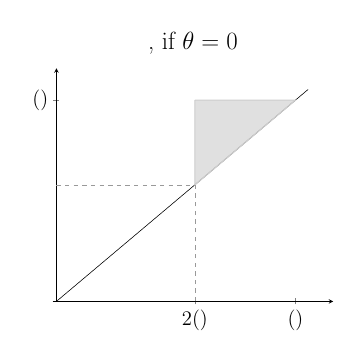
\begin{tikzpicture}[scale=0.52]
	\begin{axis} [
		title={\LARGE $\thetabarc{\cM}$, if $\img\theta_{\cM}= 0$},
		ticklabel style = {font=\Large},
		axis y line=middle,
		axis x line=middle,
		ytick={0.95},
		yticklabels={$\diam(\cM)$},
		xtick={0.55,0.95},
		xticklabels={$2\crit(\cM)$, $\diam(\cM)$},
		xmin=-0.015, xmax=1.1,
		ymin=0, ymax=1.1,]
		\addplot [mark=none] coordinates {(0,0) (1,1)};
		\addplot [thick,color=black!20!white,fill=black!30!white,
		fill opacity=0.4]coordinates {
			(0.55,0.95)
			(0.55,0.55)
			(0.95,0.95)
			(0.55,0.95)};
		\addplot [black!40!white,mark=none,dashed, thin] coordinates {(0,0.55) (0.55,0.55)};
		\addplot [black!40!white,mark=none,dashed, thin] coordinates {(0.55,0) (0.55,0.55)};
	\end{axis}
\end{tikzpicture}
	\caption{In each figure, the gray region represents where additional bars could potentially exist within the corresponding barcode.}
	\label{fig:barcodes_general}
\end{figure}
% !TEX root = ../vr_st.tex

\subsection{Spheres and their wedge sum}\label{ss:Sn}

For any integer $n \geq 1$ and real number $\rho > 0$, let $\bS^n(\rho)$ be the \defn{$n$-sphere of radius $\rho$}
\[
\bS^n(\rho) = \set{x \in \R^n \mid \bars{x} = \rho}.
\]
With the induced Riemannian metric, \(\bS^n(\rho)\) is referred to as a \defn{round sphere}.
We simplify notation writing \(\bS^n\) instead of \(\bS^n(1)\).
The constant
\[
\zeta_n = \arccos\Big(\frac{-1}{n+1}\Big),
\]
which is the diameter of an inscribed regular $(n+1)$-simplex in $\bS^n$, will play an important role.

\subsubsection{}\label{ss:critical values of Sn}

Characterizing the homotopy types of Vietoris--Rips complexes is a challenging question, even for simple spaces like the $n$-spheres.
For the circle $\bS^1$, a complete answer is provided in \cite{adamaszek2017VietorisProduct}, but for more general spheres $\bS^n$ with $n>1$, only partial results are known.

In \cite{adamaszek2018metric}, the authors introduced the Vietoris--Rips metric thickening, a metrization of the Vietoris--Rips complex that embeds the original metric space as a metric subspace. They determined the first scale parameter at which the homotopy type of the thickening of an \(n\)-sphere changes.
While this does not directly yield the homotopical radius of the \(n\)-sphere, it provides insights into its homotopy behavior and yields homological information, since the thickening shares the same homology as the original Vietoris–Rips complex \cite[Cor.~3]{gillespie2024vietoris}.

Building on the equivalence between the Kuratowski and Vietoris--Rips filtrations, the authors in \cite{lim2024vietoris} determined both the homotopical radius and the subsequent homotopy type in the Vietoris--Rips filtration of the \(n\)-sphere.

The following lemma is a consequence of these results, along with those from \cite{katz1983filling}.

\lemma
For any $m,n \in \N$ and linear cohomology operation $\theta$ we have:
\begin{enumerate}
	\item \(\crit(\bS^n) = \frac{1}{2}\zeta_n\),
	\item \(\firstdeath{m}{\bS^n} =
	\begin{cases}
		\frac{1}{2}\zeta_n & m = n, \\
		\hfil 0 & m \neq n,
	\end{cases}\)
	\item \(\firstdeath{\theta}{\bS^n} = 0\).
\end{enumerate}

\begin{proof}
	(1) By \cite[Thm.~7.1]{lim2024vietoris}, for any $0 < r \leq \zeta_n$, the space $\VR_r(\bS^n)$ is homotopy equivalent to $\bS^n$, and the homotopy type of $\VR_r(\bS^n)$ changes at $\zeta_n$.
	This implies $\crit(\bS^n)=\frac{1}{2}\zeta_n$.

	\smallskip (2) According to \cite{katz1983filling}, \(\fillrad(\bS^n) = \frac{1}{2}\zeta_n\).
	Applying \cref{ss:beta v.s. fillrad}, we obtain \(\firstdeath{n}{\bS^n} = \frac{1}{2}\zeta_n\).
	When $m\neq n$, the statement follows from the fact that the initial space in the filtration has a trivial degree $m$ reduced homology.

	\smallskip (3) We apply a similar argument as in the $m\neq n$ case of (2). The statement follows from the fact that the initial space in the filtration has trivial $\img_\theta$.
\end{proof}

\subsubsection{}\label{ss:VRSn projection}

Let \(n \in \N\) and \(r \in (0, \zeta_n]\).
From \cite[Thm.~7.1]{lim2024vietoris} we know that the spaces \(\VR_r(\bS^n)\) and \(\bS^n\) have the same homotopy type for any \(n \in \N\).
We now recall from \cite{adamaszek2018metric} a natural map that can be used to realize this equivalence.

In \cite{adamaszek2018metric}, the authors introduced the concept of Vietoris–Rips metric thickenings, which endows the Vietoris–Rips complex with a new topology.
They define the \defn{canonical projection of \(\VR_r(\bS^n)\)} as the set map
\[
f_r^n \colon \VR_r(\bS^n) \to \R^{n+1} \setminus \set{0} \to \bS^n,
\]
constructed by first mapping a formal linear combination \(\sum \lambda_i x_i\) to the corresponding point \(\sum \lambda_i x_i\) in \(\mathbb{R}^{n+1}\), followed by a radial projection onto \(\bS^n\).
Throughout this work, we do not distinguish between a simplicial complex and its geometric realization.

As mentioned in \cite{adamaszek2018metric}, the map $f_r^n$ is well-defined because, when $r \leq \zeta_n$, the map $\VR_r(\bS^n) \to \R^{n+1}$ misses the origin by the proof of \cite[Lemma 3]{lovasz1983self}.
Moreover, the authors proved that when \(\VR_r(\bS^n)\) is equipped with the metric thickening topology, the canonical projection is a homotopy equivalence.

More recently, \cite{gillespie2024vietoris} showed that the identity map between the Vietoris--Rips complex and the Vietoris--Rips metric thickening is a weak equivalence.
Consequently, the canonical projection of \(\VR_r(\bS^n)\) is also a weak equivalence for the usual Vietoris--Rips complex. By the Whitehead theorem, this weak equivalence between CW spaces is indeed a homotopy equivalence.
Thus, the canonical projection remains a homotopy equivalence when \(\VR_r(\bS^n)\) is equipped with the usual topology, as summarized by the following lemma.

\lemma
The canonical projection of the Vietoris--Rips complex \(\VR_r(\bS^n)\) is a homotopy equivalence for every $r \in (0, \zeta_n]$.

\subsubsection{}\label{ss:barcode_Sn}

We apply \cref{ss:critical values of Sn} and the barcode estimates from \cref{ss:barcode_general} to \(\bS^n\).
Using the facts that (1) the reduced homology of \(\bS^n\) has dimension one for \(m = n\) and is zero for all other values of \(m\), and (2) for any linear cohomology operation \(\theta \in \cO(\ell, m)\) with \(\ell \neq m\), \(\img \theta_{\bS^n}\) is trivial, we proceed with the estimation but omit the figure, as it is simply a special case of \cref{fig:barcodes_vs}.

\subsubsection{}\label{ss:barcodes_VS}

For $n \in \N$ and $u_1, \dots, u_n \in \N^n$, let
\[
\VS^{u_1,\dots,u_n} =
\overbrace{\bS^1\vee\dots\vee\bS^1}^{u_1} \vee\dots\vee \overbrace{\bS^n\vee\dots\vee\bS^n}^{u_n}.
\]
Using the homotopy equivalence between the Vietoris--Rips complex of a metric gluing with the wedge sum of the Vietoris--Rips complex described in \cref{ss:wedge sum}, we have the following isomorphisms of persistence modules for \(m \in \N\) and \(\theta \in \cO(\ell,m)\):
\[
\begin{split}
	\rH_m^\VR(\VS^{u_1,\dots,u_n}) &\cong \, \bigoplus_{i=1}^n \rH_m^\VR(\bS^i)^{\oplus u_i}, \\
	\img_\theta^\VR(\VS^{u_1,\dots,u_n}) &\cong \, \bigoplus_{i=1}^n \img_\theta^\VR(\bS^i)^{\oplus u_i}.
\end{split}
\]

Therefore, both the homology barcodes and \(\img_\theta\)-barcodes of \(\VR(\VS^{u_1, \dots, u_n})\) are the multiset unions of the corresponding barcodes of \(\bS^{u_i}\); see \cref{fig:barcodes_vs}.

\begin{figure}
	\centering
	\begin{tikzpicture}[scale=0.52]
	\begin{axis} [
		title = {\LARGE $\Hbarc[\field]{m}{\VS},\, u_m\neq 0$},
		ticklabel style = {font=\Large},
		axis y line=middle,
		axis x line=middle,
		ytick={0.5,0.6,0.67,0.95},
		yticklabels={,$ \zeta_m$,,$\pi$},
		xtick={0.5,0.55,0.95},
		xticklabels={ ,$\zeta_n$, $\pi$},
		xmin=-0.015, xmax=1.1,
		ymin=0, ymax=1.1,]
		\addplot [mark=none] coordinates {(0,0) (1,1)};
		\addplot [thick,color=black!20!white,fill=black!30!white,
		fill opacity=0.4]coordinates {
			(0.55,0.95)
			(0.55,0.55)
			(0.95,0.95)
			(0.55,0.95)};
		\addplot [black!40!white,mark=none,dashed, thin] coordinates {(0,0.6) (0.6,0.6)};
		\addplot [black!40!white,mark=none,dashed, thin] coordinates {(0,0.55) (0.55,0.55)};
		\addplot [black!40!white,mark=none,dashed, thin] coordinates {(0.55,0) (0.55,0.55)};
		\addplot[barccolor,mark=*] (0, 0.6) circle (2pt) node[above right,barccolor]{};%{\Large\textsf{1}};
		%\node[mark=none] at (axis cs:0.68,0.21){$\Hbarc{2}{\VS^n}$};
	\end{axis}
\end{tikzpicture}
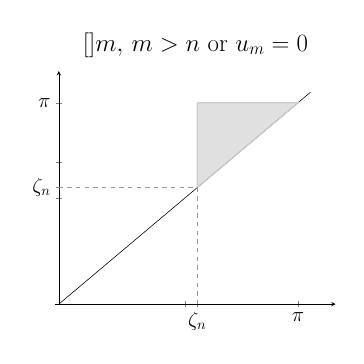
\begin{tikzpicture}[scale=0.52]
	\begin{axis} [
		title = {\LARGE $\Hbarc[\field]{m}{\VS},\, m>n$ or $u_m = 0$},
		ticklabel style = {font=\Large},
		axis y line=middle,
		axis x line=middle,
		ytick={0.5,0.55,0.67,0.95},
		yticklabels={,$\zeta_n$,,$\pi$},
		xtick={0.5,0.55,0.95},
		xticklabels={ ,$\zeta_n$, $\pi$},
		xmin=-0.015, xmax=1.1,
		ymin=0, ymax=1.1,]
		\addplot [mark=none] coordinates {(0,0) (1,1)};
		\addplot [thick,color=black!20!white,fill=black!30!white,
		fill opacity=0.4]coordinates {
			(0.55,0.95)
			(0.55,0.55)
			(0.95,0.95)
			(0.55,0.95)};
		\addplot [black!40!white,mark=none,dashed, thin] coordinates {(0,0.55) (0.55,0.55)};
		\addplot [black!40!white,mark=none,dashed, thin] coordinates {(0.55,0) (0.55,0.55)};
		%\node[mark=none] at (axis cs:0.68,0.21){$\Hbarc[\field]{m}{\VS^n}, m\geq 3$};
	\end{axis}
\end{tikzpicture}

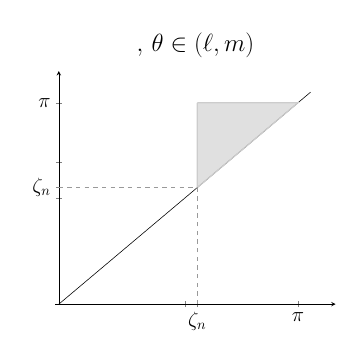
\begin{tikzpicture}[scale=0.52]
	\begin{axis} [
		title={\LARGE $\thetabarc{\VS},\, \theta \in \cO(\ell,m)$},
		ticklabel style = {font=\Large},
		axis y line=middle,
		axis x line=middle,
		ytick={0.5,0.55,0.67,0.95},
		yticklabels={,$\zeta_n$,,$\pi$},
		xtick={0.5,0.55,0.95},
		xticklabels={ ,$\zeta_n$, $\pi$},
		xmin=-0.015, xmax=1.1,
		ymin=0, ymax=1.1,]
		\addplot [mark=none] coordinates {(0,0) (1,1)};
		\addplot [thick,color=black!20!white,fill=black!30!white,
		fill opacity=0.4]coordinates {
			(0.55,0.95)
			(0.55,0.55)
			(0.95,0.95)
			(0.55,0.95)};
		\addplot [black!40!white,mark=none,dashed, thin] coordinates {(0,0.55) (0.55,0.55)};
		\addplot [black!40!white,mark=none,dashed, thin] coordinates {(0.55,0) (0.55,0.55)};
		%\node[mark=none] at (axis cs:0.68,0.21){$\sqbarc{k}{\VS^n},\, k\geq 1$};
	\end{axis}
\end{tikzpicture}

	\caption{Let $\VS = \VS^{u_1,\dots,u_n}$ for some tuple of non-negative integers.
		\emph{Top row:} persistent reduced homology barcodes of $\VS$, where the dot $(0,\zeta_m)$ has multiplicity $u_m$ which can be zero.
		\emph{Bottom row:} $\img_\theta$-barcodes of $\VS$ where $\theta \in \cO(\ell,m)$ with \(\ell \neq m\).
		In each figure, the gray region represents where additional bars could exist within the corresponding barcode.
		See \cref{ss:barcode_Sn} for the case when the wedge sum is a single sphere and see \cref{ss:barcodes_VS} for the general case.}
	\label{fig:barcodes_vs}
\end{figure}
% !TEX root = ../vr_st.tex

\subsection{General quotients}

\subsubsection{}

%An action of a group $G$ on a set $X$ is a function $G\times X\to X$ such that $g\cdot (h\cdot x)=(gh)\cdot x$, and $e\cdot x = x$ for all $x\in X$ and $g,h\in G$, where $e$ is the identity element of $G$.

Let $G$ be a group acting on a metric space $\cX$, we denote its orbit space with the quotient topology by $\cX_G$.
Orbits will be denoted as $[x]$ for $x \in \cX$.
We say the action of $G$ is \defn{proper} if, for every $x \in \cX$, there is some $r>0$ such that $\{g \mid g\cdot B(x,r) \cap B(x,r) = \emptyset\}$ is finite.
We say $G$ \defn{acts by isometries} on $\cX$, if the map $g \colon \cX \to \cX$ is an isometry for every $g \in G$.

Let $G$ be a group acting properly and by isometries on a metric space $\cX$.
Then the \defn{quotient metric}, defined by
\[
d_{\cX_G}\big([x], [x']\big) = \inf_{g \in G} d_\cX(x, g \cdot x'),
\]
is well-defined on $\cX_G$.

The action of a group $G$ on $\cX$ is said to be \defn{$r^*$-diameter}, where $r > 0$, if for any non-negative integer $k$, the condition $\diam_{\cX_G}\set[\big]{[x_0],\dots,[x_k]} < r$ implies the existence of a unique choice of $g_i$ for each $i \in \set{1,\dots,k}$ such that $\diam_{\cX}\set{x_0, g_1x_1, \dots, g_kx_k} < r$.
% \anibal{Please finish this. Why \(r \neq 0\)? Whats the quantifier: for all or there is?
% 	\ling{We need to be careful with the citation here: (1) cite \cite{adams2022metric} for the original definition; (2) cite Liam Barham for the fixed definition. We should ask Liam Barham for permission to cite his unpublished work.}}
% \anibal{I ask this below, but here is the appropriate place to answer: Does \(r^*\)-diam imply proper?}

\subsubsection{}\label{subsub:h}

A \(G\)-action on $\cX$ induces a natural \(G\)-action on the Vietoris--Rips complex $\VR(\cX)$.
Explicitly, for any \(r > 0, g\in G\) and $\sum \lambda_i x_i \in \VR_r(\cX)$,
\[
g \cdot \sum \lambda_i x_i = \sum \lambda_i (g\cdot x_i).
\]
With respect to this action, there is an induced map on orbit spaces given by
\begin{align*}
	\tilde h_r \colon \VR_r(\cX_G) &\to \VR_r(\cX)_G \\
	\textstyle\sum\lambda_i [x_i] &\mapsto \textstyle \big[\sum\lambda_i x_i\big].
\end{align*}
If the action is proper and by isometries as well as \(r^*\)-diameter, then for any \(s \leq r\), the map $\tilde{h}_s$ is a simplicial isomorphism.
This result was initially stated in \cite[Prop.~3.5]{adams2022metric} under a weaker assumption than the \(r^*\)-diameter condition.
A counterexample to the original statement and the above corrected one were provided by Liam Barham \cite{bibid}.

% \medskip\lemma
% Let $G$ act properly and by isometries on $\cX$.
% If the \(G\)-action is a $t^*$-diameter action then, for any \(s < t\), the map \((h_s)_G\) is a simplicial isomorphism.\footnote{A lot to explain here, including the assumptions, the counterexample, and the change in the notation wrt the original. Confusingly, \(h\) here is the inverse of \(\tilde h\) there.}

% \begin{proof}
% 	Because $G$ acts by isometry, we have a well-defined map
% 	\[
% 	\tilde{h} \colon \VR_r\cX \to \VR_r(\cX_G)
% 	\text{ with }
% 	\sum_{i=1}^k \lambda_i x_i \mapsto \sum_{i=1}^k \lambda_i [x_i],
% 	\]
% 	Because two points in the same orbit of the $G$ action always have the same image under $\tilde{h}$, it induces a map $\tilde{h}_G \colon (\VR_r\cX)_G \to \VR_r(\cX_G)$.

% 	Moreover, $\tilde{h}_G$ is an isomorphism, following from the fact that the action of $G$ on $\cX$ is an $r^*$-diameter action; see \cite[Proposition 3.5]{adams2022metric} for further details.
% 	Therefore, $h$, the inverse of $\tilde{h}_G$, is also an isomorphism.
% \end{proof}

\subsection{Quotients of spheres}

\subsubsection{}
\label{subsub:VR-compatible-Sn}
A \(G\)-action on \(\bS^n\) which is both proper and by isometries is said to be \defn{\(\VR\)-compatible} if, for each $r \in (0, \zeta_n]$, it commutes with the \(\VR_r(\bS^n)\)-projection (see \cref{ss:VRSn projection}) and the induced map
\[
\tilde f_r^n \colon \VR_r(\bS^n)_G \to \bS^n_G,
\]
is a weak equivalence.
For example, based on the results in \cref{ss:VRSn projection}, the trivial action is \(\VR\)-compatible.

\subsubsection{}
\label{subsub:VR-compatible-system}
An \defn{equatorial system} is a diagram
\[
\bS^{n_1} \to \bS^{n_2} \to \bS^{n_3} \to \dotsb
\]
where each arrow is an isometric embedding and $n_i \in \N$.
For example, the real and complex equatorial systems
\[
\bS^1 \subset \bS^2 \subset \bS^3 \subset \dotsb
\quad\text{and}\quad
\bS^1 \subset \bS^3 \subset \bS^5 \subset \dotsb,
\]
used for the definition of real projective (\cref{sss:cohomology_rpn}) and Lens spaces (\cref{sss:cohomology_lens}), are defined by the canonical inclusions
\[
\R^2 \subset \R^3 \subset \R^4 \subset \dotsb
\quad\text{and}\quad
\bC \subset \bC^2 \subset \bC^3 \subset \dotsb.
\]

\subsubsection{}
\label{subsub:system VR compatible}

A \defn{\(G\)-action} on an equatorial system consists of a \(G\)-action on each sphere commuting with the isometric embeddings.
For example, the group \(\rC_2 = \set{1,-1} \subset \R\) acts antipodally on the real equatorial system.
Similarly, for \(q \in \N\), the multiplicative subgroup \(\rC_q\) of \(q\)-roots of unity acts on the complex equatorial system.

We say that a \(G\)-action on an equatorial system is \defn{\(\VR\)-compatible} if the \(G\)-action on each sphere is \(\VR\)-compatible and the following diagram commutes for every \(i \in \N\) and $0 < r < \zeta_{n_{i+1}}$:
\begin{equation}\label{eq:VR_quotient}
    \begin{tikzcd}
	\VR_r(\bS^{n_i})_G
	\ar[d, hook]
	\ar[r, "\tilde f_{\,r}^{\,n_i}" above]
	&
	\bS^{n_i}_G
	\ar[d, hook]
	\\
	\VR_r(\bS^{n_{i+1}})_G
	\ar[r, "\tilde f_{\,r}^{\,n_{i+1}}" above]
	&
	\bS^{n_{i+1}}_G.
\end{tikzcd}
\end{equation}

%where
%\[
%\rho_r^n \colon \VR_r(\bS^n)_G \xra{\tilde h_r} \VR_r(\bS^n)_G \xra{\tilde f_r^n} \bS^n_G.
%\]

%\anibal{I don't know what you are proving in the hidden text below. Also, the commutativity with \(\tilde h\) should be immediate, at least on a range. Maybe the lemma below is what you want to use your proof for?}

\lemma The above \(\rC_2\)-action on the real equatorial system and the \(\rC_q\)-action on the complex one are \(\VR\)-compatible for every \(q \in \N\).

\begin{proof}
    Take any $n \in \N$ and arbitrary $0 < r \leq \zeta_{n+1} (< \zeta_{n})$.
    The commutativity of diagram \ref{eq:VR_quotient}, with $n_i = n$ and $n_{i+1} = n+1$ follows directly from the commutativity of the corresponding diagram without group actions.

    It remains to check that the group action on each sphere $\bS^n$ is \(\VR\)-compatible (see \cref{subsub:VR-compatible-Sn}), which means the group action commutes with the $\VR_r(\bS^{n})$-projection $f_r^{n}\colon \VR_r(\bS^{n}) \to \bS^{n}$ and $f_r^{n}$ induces weak equivalences on the orbit spaces.

    In the case of $\rC_2$-action on the real equatorial system, verifying that the $\rC_2$-action commutes with $f_r^{n}$ is straightforward.
    By \cref{ss:VRSn projection}, $f_r^{n}$ is a homotopy equivalence.
    Because the $\rC_2$-action is proper and free, the $\rC_2$-equivariant homotopy equivalence $f_r^n$ induces homotopy equivalence (and thus weak equivalence) on the orbit spaces.

    The case of $\rC_q$-action on the complex equatorial system follows from a similar argument.
    %In the case of the $\rC_2$-action, because $f_r^{n}$ is $\rC_2$-equivariant, the induced map $\tilde{f}_r^{n}$ is also a homotopy equivalence. \ling{This is the argument used by \cite[Theorem 4.5]{adamaszek2018metric}, but I am not sure why it is true and I am not sure if it generalizes to $\rC_m$-actions.\anibal{Since the action is proper and free, a weak equivalence equivariant wrt the action induces a weak equivalence of orbits. It is easy to see that \(f\) is equivariant wrt the \(\bS^1\) action defining the action of \(\cyc_q\)}}
\end{proof}

\subsubsection{}\label{ss:fundamental_lemma}

A \(G\)-action on an equatorial system is said to be \defn{free} if the \(G\)-action on every sphere is free.
% In this case, each orbit space is a closed manifold which is equipped with the quotient metric.

\medskip\lemma Consider a free $\VR$-compatible $G$-action on an equatorial system
\[
\bS^{n_1} \to \bS^{n_2} \to \bS^{n_3} \to \dotsb.
\]
If $\fillrad(\bS^{n_i}_G)$ is non-decreasing as a function of \(i\) then, for any \(i \leq j\),
\[
\firstdeath{n_i}{\bS^{n_j}_G} \leq \fillrad(\bS^{n_j}_G).
\]

\begin{proof}\anibal{Ling: Did we decide to use the parenthesis on VR? \ling{We did not reach a conclusion.}}
    To simplify notation, for any $i \leq j$, let
    \[
        \cX_j = \bS^{n_j}_G, \,\delta_j = \fillrad(\cX_j) \text{ and }\beta_i^j = \firstdeath{n_i}{\cX_j}.
    \]
	We will use an induction argument on $j$.
	When $j = 1$, because $\cX_1$ is connected and $n_1$-dimensional, we apply results in \cref{ss:beta v.s. fillrad} to deduce that $\beta_1^1 = \delta_1$.
	%Because $\delta_1 \leq \alpha_1$, $\rH_1(\VR\bS^1_G)$ retains the same isomorphism type before $\delta_1$, implying that $\beta_{1, 1} \geq \delta_1$.
	%Thus, $\beta_{1, 1} =\delta_1$.

	Assume the statement holds for $\cX_{j-1}$, that is, $\beta_i^{j-1} \leq \delta_{j-1}$ for any $i \leq j-1$.
	Since $\delta_{j-1} \leq \delta_j$, we have the following commutative diagram of topological spaces for any $r,\epsilon>0$ small:
    \begin{equation}\label{d:fundamental_bars_diagram}
        \begin{tikzcd}
            \cX_{j-1}
            \ar[d, hook,"{\iota}" left]
            &
            \VR_r\cX_{j-1}
            \ar[d, hook,"\iota_r" left]
            \ar[l, "\rho^{j-1}" above]
            \ar[r, hook, "v^{j-1}"]
            &
            \VR_{\delta_{j-1}+\epsilon}\cX_{j-1}
            \ar[d, hook]
            \\
            \cX_j
            &
            \VR_r\cX_j
            \ar[l, "\rho^j" below]
            \ar[r, hook, "v^j" below]
            &
            \VR_{\delta_j+\epsilon}\cX_j.
        \end{tikzcd}
    \end{equation}
    Here, the vertical maps are all induced by the equatorial inclusion of the orbit spaces $\iota \colon \cX_{j-1} \hookrightarrow \cX_j$.
    The horizontal inclusion $v^{j-1}$ (resp. $v^j$) in the right-hand-side square is the inclusion map in the corresponding Vietoris--Rips filtration.
    The horizontal map $\rho^{j-1}$ in the left-hand-side square is the composition of the following maps introduced in \cref{subsub:h} and \cref{ss:VRSn projection}, respectively:
    \[\VR_r\cX_{j-1} \xrightarrow{\tilde{h}_r}\VR_r(\bS^{n_{j-1}})_G \xrightarrow{\tilde{f}_r^{n_{j-1}}} \cX_{j-1}.\]
    The horizontal map $\rho^j$ is defined in a similar way.

    For any $i \leq j-1$, applying the degree $n_i$ reduced homology functor to diagram (\ref{d:fundamental_bars_diagram}) and using the fact that the $\rC_2$-action on the system is $\VR$-compatible (cf. \cref{subsub:system VR compatible}), we obtain a commutative diagram of vector spaces:
	for $r,\epsilon>0$ small,
	\begin{equation}\label{eq:diagram of H}
	\begin{tikzcd}[column sep = 5em]
		\rH_{n_i}(\cX_{j-1})
		\ar[d, "\cong" left]
		&
		\rH_{n_i}(\VR_r\cX_{j-1})
		\ar[d, "\rH_{n_i}(\iota_r)" left, "\cong" right, myred]
		\ar[l, "\cong" above]
        %\ar[l, "(1)" below]
		\ar[r, "\rH_{n_i}(v^{{j-1}})", myred]
		&
		\rH_{n_i}(\VR_{\delta_{j-1}+\epsilon}\cX_{j-1})
		\ar[d]
		\\
		\rH_{n_i}(\cX_j)
		&
		\rH_{n_i}(\VR_r \cX_j)
		\ar[l, "\cong"]
        %\ar[l, "(2)" above]
		\ar[r, "\rH_{n_i}(v^j)" below, myred]
		&
		\rH_{n_i}(\VR_{\delta_n+\epsilon}\cX_j).
	\end{tikzcd}
	\end{equation}

	Let $\sigma_i$ be a representative cycle for the bar $(0,\, 2\beta_{i}^{j-1})$ in $\VR \cX_{j-1}$.
	Commutativity of the left-hand-side square of diagram (\ref{eq:diagram of H}) implies that $\rH_{n_i}(\iota_r)$ is an isomorphism.
    As $r$ is arbitrarily small, we obtain that $\rH_{n_i}(\iota_r)(\sigma_i)$ creates a bar born at $0$.
	Moreover, this bar dies after $\delta_j$ as explained below.
    It follows from the induction hypothesis $\beta_i^{j-1} \leq \delta_{j-1}$ that $\sigma_i$ dies after $\delta_{j-1}$, implying that $\rH_{n_i}(v^{{j-1}})(\sigma_i) = 0$.
	Using the right-hand-side square's commutativity, we have $(\rH_{n_i}(v^j) \circ \rH_{n_i}(\iota_r))(\sigma_i)=0$, which means $\rH_{n_i}(\iota_r)(\sigma_i)$ dies after $\delta_j+\epsilon$.
    Since this holds for any \(\epsilon > 0\), we conclude that \(\beta_i^j \leq \delta_j\).

	For the case when $i = j$, apply results in \cref{ss:beta v.s. fillrad} again to get that $\beta_j^j = \delta_j$.
	This completes the proof.
\end{proof}

% !TEX root = ../vr_st.tex

\subsection{Real projective spaces}\label{s:critical_radii_rpn}

Let us now focus on the real equatorial system with the antipodal action.
We will consider every sphere \(\bS^n(2)\) to have radius 2 so the quotient \(\rp^n\) has the same diameter as \(\bS^n\).
We will consider reduced (co)homology with mod 2 coefficients.

\medskip\lemma
For \(k,n,m \in \N\) and \(\Sq^k \in \cO(m-k, m)\) we have:
\begin{enumerate}
	\item \(\crit(\rp^n) = \frac{\pi}{3}\).
	\item \(\firstdeath{m}{\rp^n} =
	\begin{cases}
		\frac{\pi}{3} & m \leq n, \\
		\hfil 0 & \text{otherwise}.
	\end{cases}\)
	\item \(\firstdeath{\Sq^k}{\rp^n} =
	\begin{cases}
		\tfrac{\pi}{3} & k \leq \frac{n-1}{2} \text{ and } \binom{m-k}{k} \text{ is odd},\\
		\hfil 0 & \text{otherwise}. \\
	\end{cases}\)
\end{enumerate}

\begin{proof}
	(1) This part is stated and proven in \cite[Thm.~4.5]{adams2022metric}.

	(2) We only need to prove for the case of $m\leq n$, since the other case follows from the definition since \(\rH_m(\rp^n) = 0\) if \(m > n\) or \(m = 0\).

    Consider the \(\rC_2\)-action on the real equatorial system \(\bS^{1}(2) \to \bS^{2}(2) \to \dotsb \to \bS^{n}(2)\), where each $\bS^{i}(2)$ is the $i$-sphere with radius $2$.
    By \cref{subsub:system VR compatible}, this system is \(\VR\)-compatible.
    By \cite{katz1983filling}, the filling radius of $\rp^i = \bS^{i}(2)_{\rC_2}$ is $\frac{\pi}{3}$ for any $i \geq 1$, which implies that $\fillrad(\rp^i)$ is non-decreasing as a function of \(i\).
    Therefore, we can apply \cref{ss:fundamental_lemma} to deduce that for any \(m \leq n\),
    \[
    \firstdeath{m}{\rp^n} \leq \fillrad(\rp^n) = \tfrac{\pi}{3}.
    \]
	On the other hand, $\firstdeath{m}{\rp^n}\geq \crit(\rp^n) = \tfrac{\pi}{3}$.
    Thus, the equality holds.

	(3) We only need a proof for the case $k \leq \frac{n-1}{2}$ and $\binom{m-k}{k}$ odd, since \(\Sq^k = 0\) otherwise.
	Because $\crit(\rp^n)=\frac{2\pi}{3}$, $\VR_r(\rp^n)$ retains the homotopy type of $\rp^n$ for $r \in (0,\tfrac{2\pi}{3})$.
    Recall from \cref{sss:cohomology_rpn} the cohomology algebra \(\rH^\ast(\rp^n; \Ftwo) \cong \frac{\Ftwo[\sigma]}{(\sigma^{n+1} = 1)}.\)
    Thus, $\Sq^k(\sigma^{m-k}) = \sigma^{m}$ generates a bar in the $\img_{\Sq^k}$-barcode that is born at $0$ and stays alive until the non-trivial class $\sigma^{m}$ dies at $\tfrac{2\pi}{3}$.
	Thus, $\firstdeath{\Sq^k}{\rp^n} \leq \tfrac{\pi}{3}$.
	On the other hand, $\firstdeath{\Sq^k}{\rp^n} \geq \crit(\rp^n) = \tfrac{\pi}{3}$.
\end{proof}

Using the above values, the estimates resulting from the analysis of \cref{ss:barcode_general} are illustrated in \cref{fig:sq barcodes}.

\begin{figure}
	\centering
	\begin{tikzpicture}[scale=0.52]
	\begin{axis} [
		title = {\LARGE $\Hbarc{m}{\rp^n},\, m\leq n$},
		ticklabel style = {font=\Large},
		axis y line=middle,
		axis x line=middle,
		ytick={0.5,0.67,0.95},
		yticklabels={$\frac{\pi}{2}$,$\frac{2\pi}{3}$,$\pi$},
		xtick={0.5,0.67,0.95},
		xticklabels={$\frac{\pi}{2}$,$\frac{2\pi}{3}$,$\pi$},
		xmin=-0.015, xmax=1.1,
		ymin=0, ymax=1.1,]
		\addplot [mark=none] coordinates {(0,0) (1,1)};
		\addplot [thick,color=black!20!white,fill=black!30!white,
		fill opacity=0.4]coordinates {
			(0.67,0.95)
			(0.67,0.67)
			(0.95,0.95)
			(0.67,0.95)};
		\addplot [black!40!white,mark=none,dashed, thin] coordinates {(0,0.67) (0.67,0.67)};
		%\addplot [black!40!white,mark=none,dashed, thin] coordinates {(0,0.72) (0.72,0.72)};
		\addplot [black!40!white,mark=none,dashed, thin] coordinates {(0.67,0) (0.67,0.67)};
		\addplot[barccolor,mark=*] (0, 0.67) circle (2pt) node[above right,barccolor]{};%{\Large\textsf{1}};
		%\node[mark=none] at (axis cs:0.68,0.21){$\Hbarc{1}{\rp^n}$};
	\end{axis}
\end{tikzpicture}
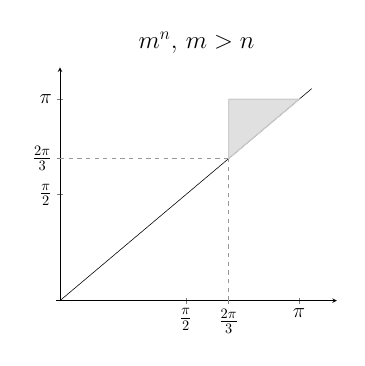
\begin{tikzpicture}[scale=0.52]
	\begin{axis} [
		title={\LARGE $\Hbarc{m}{\rp^n},\, m>n$},
		ticklabel style = {font=\Large},
		axis y line=middle,
		axis x line=middle,
		ytick={0.5,0.67,0.95},
		yticklabels={$\frac{\pi}{2}$,$\frac{2\pi}{3}$,$\pi$},
		xtick={0.5,0.67,0.95},
		xticklabels={$\frac{\pi}{2}$,$\frac{2\pi}{3}$,$\pi$},
		xmin=-0.015, xmax=1.1,
		ymin=0, ymax=1.1,]
		\addplot [mark=none] coordinates {(0,0) (1,1)};
		\addplot [thick,color=black!20!white,fill=black!30!white,
		fill opacity=0.4]coordinates {
			(0.67,0.95)
			(0.67,0.67)
			(0.95,0.95)
			(0.67,0.95)};
		\addplot [black!40!white,mark=none,dashed, thin] coordinates {(0,0.67) (0.67,0.67)};
		\addplot [black!40!white,mark=none,dashed, thin] coordinates {(0.67,0) (0.67,0.67)};
		% \addplot[barccolor,mark=*] (0, 0.67) circle (2pt) node[above right,barccolor]{\Large\textsf{1}};
		% \node[mark=none] at (axis cs:0.68,0.21){$\Hbarc{m}{\rp^n},\, m\geq 2$};
	\end{axis}
\end{tikzpicture}

\begin{tikzpicture}[scale=0.52]
	\begin{axis} [
		title = {\LARGE $\sqbarcl{k}{}{\rp^n},\, m \leq n$ and $\binom{m-k}{k}$ odd},
		ticklabel style = {font=\Large},
		axis y line=middle,
		axis x line=middle,
		ytick={0.5,0.67,0.95},
		yticklabels={$\frac{\pi}{2}$,$\frac{2\pi}{3}$,$\pi$},
		xtick={0.5,0.67,0.95},
		xticklabels={$\frac{\pi}{2}$,$\frac{2\pi}{3}$,$\pi$},
		xmin=-0.015, xmax=1.1,
		ymin=0, ymax=1.1,]
		\addplot [mark=none] coordinates {(0,0) (1,1)};
		\addplot [thick,color=black!20!white,fill=black!30!white,
		fill opacity=0.4]coordinates {
			(0.67,0.95)
			(0.67,0.67)
			(0.95,0.95)
			(0.67,0.95)};
		\addplot [black!40!white,mark=none,dashed, thin] coordinates {(0,0.67) (0.67,0.67)};
		%\addplot [black!40!white,mark=none,dashed, thin] coordinates {(0,0.72) (0.72,0.72)};
		\addplot [black!40!white,mark=none,dashed, thin] coordinates {(0.67,0) (0.67,0.67)};
		\addplot[barccolor,mark=*] (0, 0.67) circle (2pt) node[above right,barccolor]{};
        %{\Large$\geq$\textsf{1}};
	\end{axis}
\end{tikzpicture}
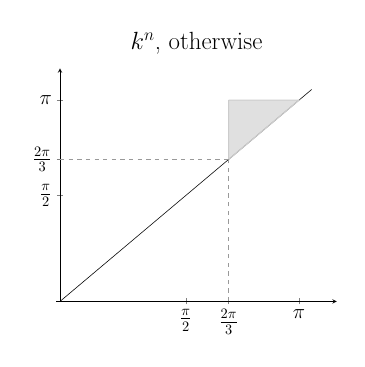
\begin{tikzpicture}[scale=0.52]
	\begin{axis} [
		title={\LARGE $\sqbarcl{k}{}{\rp^n}$, otherwise},
		ticklabel style = {font=\Large},
		axis y line=middle,
		axis x line=middle,
		ytick={0.5,0.67,0.95},
		yticklabels={$\frac{\pi}{2}$,$\frac{2\pi}{3}$,$\pi$},
		xtick={0.5,0.67,0.95},
		xticklabels={$\frac{\pi}{2}$,$\frac{2\pi}{3}$,$\pi$},
		xmin=-0.015, xmax=1.1,
		ymin=0, ymax=1.1,]
		\addplot [mark=none] coordinates {(0,0) (1,1)};
		\addplot [thick,color=black!20!white,fill=black!30!white,
		fill opacity=0.4]coordinates {
			(0.67,0.95)
			(0.67,0.67)
			(0.95,0.95)
			(0.67,0.95)};
		\addplot [black!40!white,mark=none,dashed, thin] coordinates {(0,0.67) (0.67,0.67)};
		\addplot [black!40!white,mark=none,dashed, thin] coordinates {(0.67,0) (0.67,0.67)};
	\end{axis}
\end{tikzpicture}
	\caption{Let $m \in \N$ and $\Sq^k \in \cO(m-k, k)$.
        \emph{Top row:} the persistent reduced homology barcode of $\rp^n$.
		%When $1\leq \degp \leq n$, the barcode consists of one $(0,\frac{2\pi}{3})$ and potentially some bars dominated by $(\frac{2\pi}{3}, \pi)$.
		\emph{Bottom row:} the $\img_{\Sq^k}$-barcode of $\rp^n$.
		%The leftmost barcode contains at least one $(0,\frac{2\pi}{3})$ and potentially some bars dominated by $(\frac{2\pi}{3}, \pi)$;
        %See \cref{s:critical_radii_rpn} for details.
        In each figure, the gray region represents where additional bars could exist within the corresponding barcode.
	}
	\label{fig:sq barcodes}
\end{figure}

\subsection{Lens spaces}\label{s:critical_radii_lens}

Much less information is known about Lens spaces.
We are interested in spheres \(\bS^{2n+1}(p)\) of radius \(p\), so the quotient \(\rL_p^n\) has the same diameter as \(\bS^{2n+1}\).
We will consider reduced (co)homology with mod \(p\) coefficients.

\medskip\lemma 
For fixed $n\in \N$, if $\fillrad(\rL^1_p) \leq \dotsb \leq \fillrad(\rL^n_p) < \tfrac{3\zeta_{2n+1}}{4}$, then for any non-negative degree $m\leq 2n+1$, 
\[
\firstdeath{m}{\rL^n_p} \leq \tfrac{\zeta_{2n+1}}{4} + \tfrac{\zeta_{m}}{2}.
\]

\begin{proof}
    It is enough to consider odd homology degrees, since $\firstdeath{m}{\rL^n_p} = 0$ when $m$ is even.
    For odd degrees, we apply an argument similar to that in the second part of the proof of \cref{s:critical_radii_rpn}.
    By \cref{subsub:system VR compatible}, the $\rC_p$-action on the system $\bS^1(p) \subset \bS^3(p) \subset \dotsb \subset \bS^n (p)$ is \(\VR\)-compatible. \ling{verify the consistence of radius}
    This, combined with the assumption that $\fillrad(\rL^{n'}_p)$ is non-decreasing in $n'$ for all $1\leq n' \leq n$, meets the conditions of \cref{ss:fundamental_lemma}, implying that for any odd integer $m \leq 2n+1$,
    \[
    \firstdeath{m}{\rL^n_p} \leq \fillrad(\rL^n_p) \leq \tfrac{3\zeta_{2n+1}}{4} \leq \tfrac{\zeta_{2n+1}}{4} + \tfrac{\zeta_{m}}{2}. \qedhere
    \]
\end{proof}


-------------------------\anibal{Please make a statement here that can be used to check Desideratum (2) later. I am guessing something like the fundamental lemma. Then in the Desiderata section one would just reference this. \ling{done.} }